



\section{Theoretical Foundations}

This chapter examines the individual components of this reasearch. It starts with a deeper look at stress and its impact on the Autonomic Nervous System, followed by a discussion on heart rate and heart rate variability. Moreover, the concept of rPPG, the mechanism of biofeedback, and the influence of music on stress regulations are investigated.

\subsection{Stress and the Autonomic Nervous System}

The Autonomic Nervous System (ANS) consists of the parasympathetic and the sympathetic branches. The paraympathikus system act during periods of rest and calm and regulates functions such as “rest and digest”. In contrast, the sympathetic system is activated situations in which we precive a threat. In these cases, the heart rate increases to release more energy \cite{mccorry2007physiology}.

McEwen (2007) describes this as the allostatic effect. The body dynamically adjusts its internal state to meet the standards of the environment. For instance, in a life threatening situation a lot of energy is released. The short-term mobilization of energy is a protective reaction of the body. If this activation occurs chronically without enough recovery, it can lead to permenant damage (Figure \ref{fig:allostatic_load}) \cite{mcewen2017neurobiology}.

Individual differences in stress perception are rooted in the brains’ ability to evaluate environmental stimuli. According to McEwen (2007), the brain exhibits significant plasticity, meaning its responses to stressors is shaped by genetics, early development, and past experiences. If an individual has for example experiences a trauma, the brain’s system may become hypersensitiv. It might trigger a ‘fight or flight’ response in harmless situations. This can lead to coping strategies, such as smoking or drinking. These coping stragies try to calm down the parasympathetic branch of the autonomic Nervous System. On the other hand, the plasticity also allows for an intervention in the other direction. The brain can be trained to shift from a threatening state to a calm state \cite{mcewen2017neurobiology}.

\begin{figure}[!ht]
    \centering
    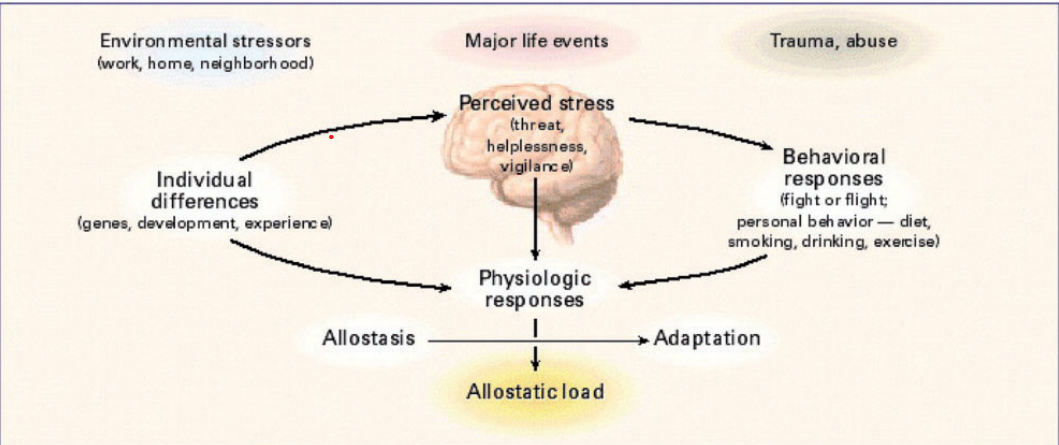
\includegraphics[width=0.9\columnwidth]{./chapters/pictures/test.png}
    \caption{The Figure illustrates the mechanism of allostatic load and the underlying pathways of stress perception and physiological adaption. \cite{mcewen2017neurobiology}}
    \label{fig:allostatic_load}
\end{figure}


\subsection{Heart Beat and Heart Rate Variability}

To understand the mechanics of stress detection, it is essential to differentiate between the quantity and the quality of heart activity. These two aspects are represented by Heart Rate (HR) and Heart Rate Variability (HRV) \cite{shaffer2017overview}.

Heart Rate (HR) is defined as the total number of heartbeats per minute. It acts as a measure of how fast the heart is beating at any given moment. It remains a relatively coarse metric. For instance, in an office environment, HR often stays within a specific range, as there is not enough physical activity. This can make it an insensitive marker for subtle cognitive loads or early-stage stress \cite{shaffer2017overview}.

Heart Rate Variability (HRV), on the other hand, focuses on the smaller level of cardiac timing. It describes  the fluctuation in the time intervals between two heartbeats. This is defined as Interbeat Intervals (IBIs). HRV consists of the constant changes in these time intervals from one beat to the next \cite{shaffer2017overview}.

From a physiological standpoint, a healthy biological system requires to be highly adaptable. This means that a healthy heart does not maintain a perfectly rigid or identical time between intervals. Instead, the autonomic nervous system constantly changes the timing of each beat to respond to internal and external demands \cite{shaffer2017overview}.

% hier vielleicht noch ein wenig kürzer das ist schon sehr viel text (hier nochmal nach AI schauen)
If the intervals between heartbeats become too consistent and lose this natural irregularity, it is often a clinical sign of physiological strain or a lack of regulatory flexibility. High variability indicates that the body is in a state of balance and can rapidly adjust to stressors. Therefore, while HR measures the quantity of beats, HRV reflects the quality and efficiency of the autonomic nervous system’s control over the cardiovascular system \cite{shaffer2017overview}.


\subsection{Remote Photoplethysmography (rPPG)}

To measure the heart beat and the heart beat variability a technology called remote Photoplethysmography can be employed.

\subsubsection{The foundations of rPPG}

The foundational work for modern remote photoplethysmography (rPPG) was made by Verkruysse et al. (2008), who demonstrated that the heart beat could be monitored using a standard digital camera. This relies on the fact that hemoglobin absords light differently than the surrounding body tissue. As the blood volume changes in the body with every heartbeat, the intensity of the reflected light varies. Their research identified that the green color channel contains the strongest information regarding the heart beat (Figure \ref{fig:blood_frequencies}). Despite the successful proof-of-concept, two challenges were highlighted: Motion artifcats caused by movement and  noise due to the camera's sensor \cite{verkruysse2008remote}.

\begin{figure}[!ht]
    \centering
    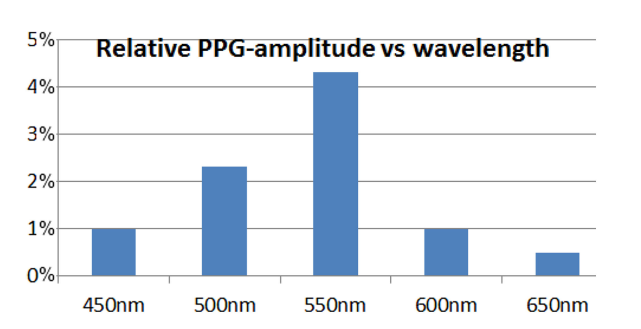
\includegraphics[width=0.9\columnwidth]{./chapters/pictures/blood_frequencies.png}
    \caption{Spectral sensitivity of the PPG signal. Green light exhibits the highest amplitude, making it the most reliable channel for non-contact heart rate monitoring. \cite{dehaan2013chrom}}
    \label{fig:blood_frequencies}
\end{figure}

\subsubsection{Evolution: From Classic Algorithms to AI-based Detection}

Following the initial proof-of-concept, a significant increase in rPPG research was observed, particularly after 2017. This trend is closely linked to the rapid improvements in Artificial Intelligence (AI) and Deep Learning. A recent meta-analysis revealed that in 2025 82.05\% \cite{Debnath25} of papers about rPPG technology used an approach with artificial intelligence. A major problem is the availability of diverse, large-scale datasets. The available sets only have data of people from North America, Europe and China. This leads to a huge underrepresentation of various age groups and diverse skin tones \cite{Debnath25}.


\subsubsection{Tradtional Frameworks and Region of Interest (ROI)}

Traditional rPPG frameworks typically follow a multi-stage process. First, the face is detected and tracked, often using the Viola-Jones algorithm or similar cascade classifiers to define a Region of Interest (ROI). Then methods such as Principal component Analysis (PCA) or Independet Component Analysis (ICA) or employed to isolate the pulse signal from the green color channel. While effective if the person remains still, these approaches struggle with motion artifacts, as they require several seconds of stable data to compute the signal components \cite{Debnath25}.

While traditional frameworks rely on fixed mathematical models, modern approaches increasingly replace stages of the rPPG pipeline with Deep Learning modules. This is done in the area of face detection and tracking. The Viola-Jones algorithm often struggles with varying lighting conditions and extreme head poses. Current systems frequently utilize more robust AI-based detectors \cite{Debnath25}.

Furthermore, the region of interest (ROI) significantly impact the accuracy of the heart rate. Although, early studies often used the entire facial area, recent studies recommend using a small rectangular area at the forhead for better results \cite{Debnath25}.


\subsection{Blind Source Separation}

The fundamental problem in rPPG is that the recorded RGB channels do not only contain the pulse information but also significant noise in the form of light changes and movement. The challenge is that this noise has to be separated from the real physiological information. Mathematically speaking, the resulting color channels are treated as a linear mixture \cite{poh2010non} :

$$x(t) = As(t)$$

The goal is to find a demixing matrix $W$, so that the original source signals $\hat{s}(t) = Wx(t)$ can be calculated. To find $W$, it is important to search for statistical independence between the sources. For that, the JADE algorithm (Joint Approximate Diagonalization of Eigenmatrices) is used. Unlike deterministic methods, JADE is an iterative process that tries out different combinations to maximize non-Gaussianity, which results in a higher computational load and increased latency (Figure \ref{fig:color_channels}) \cite{poh2010non}.

\begin{figure}[!ht]
    \centering
    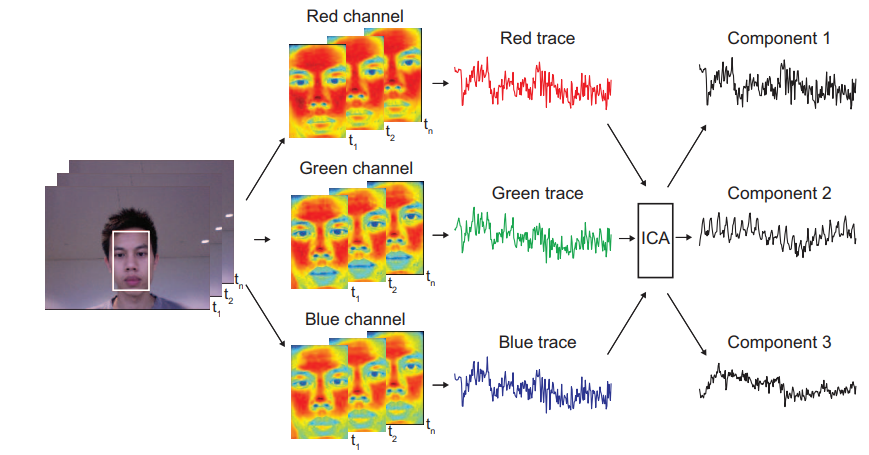
\includegraphics[width=0.9\columnwidth]{./chapters/pictures/color_channels.png}
    \caption{Seperation of color channels \cite{poh2010non}}
    \label{fig:color_channels}
\end{figure}


For the initial localization, the Viola-Jones algorithm is used to detect the face. In this specific setup, only 60\% of the bounding box width is used as the Region of Interest (ROI). The raw signals from this ROI are then spatially averaged and normalized using Zero-Mean and Unit-Variance to balance different channel intensities \cite{poh2010non}.

After the independent components are recovered, the pulse is extracted by using the Fast Fourier Transform (FFT). An operational range from [0.75 - 4.0] Hz is allowed, because this corresponds to 45 - 240 BPM, the range a human pulse usually lies in. Additionally, a temporal consistency threshold is implemented: a jump of only 12 BPM is allowed between consecutive measurements (taken 1 s apart). Anything different is rejected as noise or an artifact. The highest power peak within the frequency spectrum is chosen as the final heart rate \cite{poh2010non}.

To compare the accuracy of this methodology to a gold standard (like a finger BVP sensor), Bland-Altman plots are used. These plots show that ICA can significantly reduce the Root Mean Squared Error (RMSE) from 19 BPM to about 4.6 BPM even when the subject is moving \cite{poh2010non}.

However, there are physical limitations to consider. According to the Beer-Lambert Law, the way light travels through and is absorbed by blood vessels is technically non-linear. But for the sake of computation, ICA uses a linear approximation, which works well for short time windows (e.g., 30s). The system is also highly dependent on the ambient lumination; if it is too dark, the SNR drops too low for a reliable measurement \cite{poh2010non}.

Another risk is the "Component Picking" problem. In this study, the second independent component is usually chosen as the pulse signal because hemoglobin absorptivity is highest in the green spectrum. However, this fixed selection could be wrong if the noise is too strong. Finally, it is noted that using simple webcams is much more cost-effective than using expensive thermal cameras, and the software-based approach even allows for the simultaneous detection of multiple people in one frame \cite{poh2010non}.


% hier umschreiben
% iterative functions are used to maximize or minimize a given cost function that measures non-Gaussiannity

% at the end fast Fourier transform (FFT)

% operational range to [0.75, 4]

% threshold for maximum change in pulse rate between successive measurements maximum threshold of 12

% cardiovascular pulse wave was clearly visible in the second component

% false positive and false negative was 0\%


% free to move their head or body slowly while remaining seated


% simultaneous heart rate measurements

% ICA(30s ) used
% linear model should provide a reasonable local approximation -> the results confirm that removing noise in these situations

% primary use of this methodology likely to be in a home environment

% jeder farbsensor (RGB) nimmt eine Mischung aus dem Puls und Störquellen auf (Licht, Bewegung) aufnimmt

% es wird der Jade algorithmus benutzt -> hier wird viel ausprobiert und daher hat man eine höhere rechenzeit

% Viola-Jones Algorithmus

% Zero-Mean / Unit-Variance Normalisierung -> damit die unterschiedlichen Helligkeiten der Farbkanäle die ICA nicht verfälschen

% ICA gibt drei Kanäle zurück, weiß aber nicht welcher der Puls ist, Meistens ist es die zweite Komponente

% Fast Fourier Transformation (FFT) wird genutzt, um vom Zeitsignal in das Frequenzspektrum zu kommen -> 0,75HZ bis 4HZ Alles unter 45 BPM
% -> algorithmus sucht den höchsten peak in diesem bereich

% noise manchmal springt das system es wird ein limit gesetzt für die maximalen sprünge

% bland altman plots fehler wird von 6BPM auf 2.29BPM reduziert.

% das licht reist unterschiedlich tief in das Gewebe ein (Beer-Lambert-Gesetz) -> eignetlich ein nicht linearer Prozess. (ICA) geht von einer linearen mischung aus

% lineare Annäherung von 30s oder 5s reichen tehcnisch aus, um präzise ERgebnisse zu liefern.

% Vergleich mit Wärmebildkamera -> läuft auf jedem Laptop

% sie wissen nicht ob das System im Dunklen funktioniert

% man weiß nicht welche komponente die grüne farbkomponente ist.









\subsubsection{Chrom approach}

%  den abschnitt nocheinmal prüfen

The Chrominance-based method (CHROM) introduced a physicsbased alternative. It solves the big challenge of subject motion, when calculating the heart beat. Periodic movements can render simple intensity-based selections useless. Furthermore, while many algorithms require long observation intervals to achieve sufficient frequency resolution, CHROM is designed to be highly efficient. Similarly to traditional methods like PCA or ICA, the chrom algorithm also uses the fact that the blood absorb a large percentage of green light. Additionally it analyzes how the light is reflected on the human skin. According to the dichromatic reflection model this reflection has a Specular and a Diffused Component (Figure \ref{fig:chrom_light}). Only the diffuse Reflexion enters the skin and has the color of the blood. The specular reflexion does not enter the skin. It is just reflected on the surface and thus does not contain any information about the blood. This specular part is an additive value and thus the division of the two  color channels does not cancel this effect out. Thereforce, a subtraktive approach is used \cite{dehaan2013chrom}.

$$(R + noise) - (G + noise) = R - G$$


\begin{figure}[!ht]
    \centering
    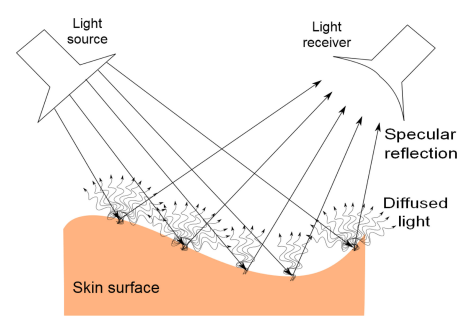
\includegraphics[width=0.9\columnwidth]{./chapters/pictures/chrom_light.png}
    \caption{The illustration depicts light reflection on the skin \cite{dehaan2013chrom}}
    \label{fig:chrom_light}
\end{figure}

The CHROM algorithm projects the normalized RGB signals into two orthogonal chrominance signals, $X$ and $Y$. In a perfect environment under white light, these signals are mathematically independent. Based on empirical data from a diverse set of subjects, de Haan and Jeanne derived the standardized projection vectors $[0.7682, 0.5121, 0.3841]$, leading to the core transformations:

$$X_s = 3R_n - 2G_n$$

$$Y_s = 1.5R_n + G_n - 1.5B_n$$

To further refine the pulse signal $S$, these components are combined using the ratio of their standard deviations ($\alpha$):

$$S = X_s - \alpha \cdot Y_s \quad where \quad \alpha = \frac{\sigma(X_s)}{\sigma(Y_s)}$$

Even after projection, the signal $S$ may contain a slow "drift" caused by respiration or minor posture changes. To isolate the cardiac signal, a Bandpass Filter is applied. The filter is typically tuned to a range of 0.7 Hz to 4.0 Hz, which corresponds to a human heart rate between 42 and 240 BPM. Frequencies outside this window are discarded as non-physiological noise.To extract the final heart rate, a Fast Fourier Transform (FFT) is performed on the filtered signal. The FFT shifts the data from the time domain to the frequency domain, resulting in a power spectrum. The algorithm identifies the "dominant peak" (the highest frequency component) in this spectrum. For instance, a peak at 1.2Hz is converted to the final pulse rate:

$$1.2 Hz \times 60 seconds = 72 BPM$$


One of the most significant advantages of CHROM is its temporal efficiency. While traditional BSS methods (Blind Source Separation) like ICA or PCA often require up to 30 seconds of data to stabilize, CHROM utilizes an Overlap-Add (WOLA) procedure. By using overlapping windows of only 1.6 seconds, the system provides a continuous, near-instantaneous pulse estimate.

In comparative studies, the robustness of CHROM is evident. CHROM has a high stationary accuracy and predictes the correct pulse with a 98\% accuracy. It has a 92\% correlation with the medical-grade contact sensor. Furthermore, it is resilient against motion. Under havey motion (e.g., on a fitness stepper), maintains a 48\% success rate. ICA and PCA fail significantly, and only reach 4\% and 11\%. Moreover, CHROM can also process different skin tones. Darker Skin Tones naturally lower the Signal-to-Noise Rratio because the absord more light. Chrom remains the most robust classical algorithm across all phenotypes.

\subsubsection{Modern Deep Learning Paradigms}

With the rapid advancement in artificial intelligence, modern rPPG systems have shifted towards end-to-end models. These architectures can process raw data or image sequences to estimate heart rate directly, often without the need for manual face isolation or region of intrest  selection. There are three architectural paradigms: Convolutional Neural Networks (CNNs), Hybrid Neural Networks and Transformed-based architectures \cite{Debnath25}.

In modern rPPG systems, Convolutional Neural Networks (CNNs) are the standard for processing image data. These networks consist of several layers, mainly an input, an output, and various hidden layers like convolutional and pooling layers. Their main task is to recognize the very subtle color changes in the skin pixels that happen during a cardiac cycle \cite{Debnath25}.

A big problem in this field, is that there aren't enough large and diverse datasets to train these models from scratch. Because of this, researchers often use Transfer Learning \cite{Debnath25}. The idea here is to take a model that was already trained on a different task, such as general face recognition. By 'freezing' the first layers and only fine-tuning the last ones with rPPG-specific data, the model can use its existing knowledge of facial features. This approach makes it possible to get good results even with smaller datasets and saves a lot of training time \cite{pan2009survey}.

In addition, a different category of neural networks has emerged: Hybrid Neural Networks. These combine different neural networks like CNNs, RNNs and autoencoders to form a more robust system \cite{Debnath25}.

In the past years powerful Large Language Models (LLMS) like ChatGPT have emerged that use transformers to understand words and sentences. The same technique can be employed to analyze pictures. The picture is broken up into small rectangular patches, which the network analyzes in relation to one another \cite{dosovitskiy2021an}. By Comparing different regions simultaneously, the transformer is able to differentiate between the heart beat and noise, such as micro-movements. This leads to a more robust heart rate estimation \cite{Debnath25}.


\subsubsection{Summary of rPPG Frameworks}
There are lot of different approaches to calculate the heartbeat with an rPPG technique.
Modern Deep Learning Algorithms have emerged in the recent years. They show promising results, although there are not enough diverse datasets. The CHROM Algorithms is promising for a realtime evaluation of data. Traditionally algorithms like PCA are slow and not so precise.
Although, there has been a huge advancement in the past years, there are still no long-term studies that monitor the heart beat over several hours. Most researches only test rPPG for a short time, which does not show how it works in real daily life \cite{Debnath25}.


\subsection{sonification}

% To create sound out from a heart beat, a transformation is required. This is defiend as sonification. According to Hermann (2008) this is a systematic transformation of data relations into acoustic signals. The purpose is information communication. Four conditions have to be met for this transformation: It has to be objective, be based on a systematic transformation, to be reproducible and be applicable to different datasets \cite{hermann2008taxonomy}.

Dubus et al. (2013) performed a systematic review on sonification. They mention that sonification can enhance the perception of one's own body and is therefore widely used in rehabilitation and training. Among different sonification techniques, parameter mapping is especially promising because it allows for continuous transmission of information. In this process, a certain set of mappings between "physical dimensions" and "auditory dimensions" is defined \cite{dubus2013systematic}.

% heir dann noch die quellenangabe raus nehmen aus [50]
To establish these mappings, a three-stage process is required. First, the specific auditory dimensions to be used must be identified, such as pitch or timbre. Then the polarity has to be defined. This determines the direction in which the auditory dimension changes according to the data. For instance, if the heart rate increases, it must be decided whether the pitch should increase or decrease. Finally, the psychophysical scaling has to be addressed. Since humans perceive changes in sound non-linearly, it is necessary to define the magnitude of the auditory change relative to the data change \cite{dubus2013systematic} \cite{walker2000psychophysical}.

According to Dubus and Bresin (2013), many sonification approaches implement a strategy called "ecological perception". This means that certain sonification principles are part of our subconscious mind. This applies, for example, to loudness, which can be explained by the inverse distance law: a decrease in sound intensity is naturally associated with an increasing distance from a source. Such natural associations are deeply ingrained in human perception and should be prioritized when employing a sonification approach \cite{dubus2013systematic}.

Research has shown which auditory dimensions are preferred in specific fields. For the dimension "Time", timbre is often used, whereas loudness is used less frequently. In the category of "Kinetics", which describes energy or force, loudness is the most common mapping. These categories are particularly relevant when sonifying the human heartbeat. Furthermore, in real-time sonification, a mapping from "instant to instant" occurs, meaning the rhythm of the underlying data source is directly incorporated into the auditory output. Additionally, data related to horizontality is more often depicted through spatialization, while vertical data is frequently sonified through pitch \cite{dubus2013systematic}.

Furthermore, it is pointed out that the sonic material is decisive. If the sounds make the user uncomfortable, this can have drastic consequences for the effectiveness of the system. Therefore, the use of sample-based displays is often preferred over simple synthetic tones \cite{dubus2013systematic}.

In addition, it is important to investigate the chosen sonification strategy scientifically. The study highlights that many approaches are currently chosen in an ad hoc or arbitrary manner without verifying their effectiveness through objective tests \cite{dubus2013systematic}.


% pitch is most used
% sonification is great to feel the own body
% great for rehabilitation and training

% different sonification techniques
% audification, parameter mapping

% parameter mapping is widely used
% information is transmitted in a continous matter

% parameter mapping: three stages
% choice of mapping strategy (which auditory dimension to use to represent a specific data dimnesion)

% choice of polarity
% choice psychological scaling

% Hypothesis 1. A large proportion of sonification mappings
% follow the logic of ecological perception. Mappings are often
% performing a sort of simulation of underlying physical phenomena,
% which can be implemented either directly or metaphorically.
% These natural associations between sound and its meaning
% regarding physics were called ‘‘universal relationships’’ by Hermann
% and Ritter [69] and depicted as ‘‘deeply engrained in the way we —
% usually subconsciously — pick up meaning from sound events’’ -> sound funktioniert am besten wenn es ökologisch ist

% All the other (i.e. not involving Pitch) mappings but one
% correspond to natural perceptual associations, which supports
% Hypothesis 1.

% Loudness can be explained by the inverse distance law: damping of sound waves in the transmission medium (e.g. air)
% leads to a decrease of sound intensity that is proportional to the
% distance to the sound source, and therefore to a decrease of
% loudness.

% Benutzte auditory dimensions: Loudness, Duration, Spatialization

% Dimension Time: Klangfarbe wird oft genutzt, Lautstärke eher weniger und Spatial eigentlich nie  (Sound der denn Klang heller dumpfer macht genutzt)

% Kinetics -> Herzrate als Anspannugn oder als Energie Kinetics es wird oft Laustärke genutzt

% Pitch ist für alle Daten möglich

% Spatial sachen werden selbst in profi projekten nie bentuzt und sind daher nicht nötig

% mapping from instant to instant -> durch den herzschlag hat man automatisch schon den rhythmus den herzes in dem song drinne

% oft werden die sonification strategies nicht wissenschaftlich getestet sondern es wird einfach ein wenig random gemacht

% We can observe that physical dimensions
% related to horizontality are most often sonified through Spatialization, while those related to verticality are most often sonified via
% changes in Pitch.

% das projekt würde zur kategorie monitoring gehören

% die art des klangmaterials ist entscheidenend und kann das experimetn maßgeblich beieinflussen

% Sample-based displays

% die meisten projekte nutzen natürliche assoziationen






\subsection{Mapping of heart beat to music}

% den abschnitt nocheinmal prüfen 

RPPG Techniques provide the functionality to measure the heart beat remotely. These measurements then need to be converted to music.

There has been some research on passive music listening without any biofeedback mechanism. According to a meta-analysis by  Pelletier(2004), music consistently assists in lowering stress levels. The magnitude of this response is affected by several factors. Patients with prior musical experience, such as playing an instrument, tend to lower their stress levels a lot more.
Furthermore, Pelletier notes that indivudal therapy generally results in better relaxation than group session. Although, group sessions are used much more often because they are less expensive. A huge obstacle is that the devices that are used for data collection often cause discomfort. This can lead to false data regarding the relaxation process. Finally, the study suggests that music based on scientific research (e.g., specific rhythmic or frequency patterns) is more effective for stress reduction that music chosen soley based on personal preference \cite{pelletier2004effect}.
In another study, Linnemann et al. examined how music affects stress in daily life rather than in a laboratory. They came to the conclusion that listening to music can effectively reduce stress levels. Nevertheless, the largest effect is reached when subjects listen to music with then intention of decreasing stress levels. This suggests that the reason why someons listens to music is very important for the actual stress-reducing effect \cite{linnemann2015music}.

These results are also supported by another study \cite{thoma2011listening}. They confirm that listening to music alone does not automatically decrease stress levels. Instead,  the reason of listening to the music is the most important factor. For example, if someone listens to music to cope with loneliness, it might effectively decrease their feeling of isolation. Nevertheless, if the goal is relaxation, the music only works well if the listener has the specific intention to relax \cite{thoma2011listening}.

The study of Bernardi et al. (2006) confirms that the results do not depend on the music preferation of the user rather on the BPM and rhythm structure of the music. Additionally, the study found no evidence of habituation, meaning the users do not simply 'get used' to the music over time. In Contrast to Linnemann et al. (2015), who emphasized the importance of the listener's intention, Bernadi concludes that music can be perceived as a passive form of meditaiton. consequently, this means that the user does not need an intend to reduce stress for measurable results \cite{bernardi2006cardiovascular}.

Passive music listening without any biofeedback system has mixed results. To convert the heartbeat to music, a process called mapping is necessary, that takes the input data and transforms it into music. There are two methods Continous mapping and diskrete mapping. Continous mapping describes the process of constantly changing the music according to the data. During the discrete mapping process certain aspects of the music are changed when a certain threshold is reached \cite{bergstrom2014using}.

\subsubsection{Biofeedback-Driven Regeneration}

As explained previously the heart rate is converted to a piece of music. It is now crucial to understand how the music can help the human body to regenerate. According to Lehrer and Gevirtz (2014), the efficiency of biofeedback relies on the synchronization of the cardiovascular and respiration systems \cite{lehrer2014heart}.

The human cardiovascular system has a certain resonance frequency at which point it exhibts the best effects on the human body. If this state is reached, has maximum internal order and physiological efficiency. This frequency is reached at approximately 0.1 Hz. This is equivalent to roughly six breaths per minute. By breathing at the resonance frequency, heart rate and blood pressure enter a harmonic state. Furthermore, gas exchange in the lungs are also optimised at this state \cite{lehrer2014heart}.

In addition, the activity of the vagus nerve is stimulated. The vagues nerve is responsible for the communication between the heart and the blood. This makes it possible for the body to lower the heart rate more effectively \cite{lehrer2014heart}.

Moreover, biofeedback creates a meditative effect that changes the user's state of consciousness. The user has to focus his thoughts and his energy on the biofeedback signal. Thus, it the brain cannot focus on anxious thoughts \cite{lehrer2014heart}.

\subsection{Consciousness and State Regulation}

The meditative effect of focusing on one's heart rate or respiration can be used to enhance consciousness. This process is frequently described through the concept of mindfulness. This makes it possible for individuals to develop a sensitivity to their thoughts and emotional states. Bishop et al. (2004) established this definition. A fundamental requirements is described as the 'non-judgemental-approach", meaning. This means that internal states are perceived with curiosity and openness. Internal thoughts and feeling should be accepted as they are \cite{bishop2004mindfulness}.


